%%%%%%%%%%%%%%%%%%%%%%%%%%%%%%%%%%%%%%%%%%%%%%%%%%%%%%%%%%%%%%%%%%%%%%%%%%%%%%%%%%%%%%%%%%%%%%%%%%%%
% Preambula

%\documentclass[14pt]{article}              % komanda nedarbojas Overleaf platformā
\documentclass[a4paper,12pt]{extarticle}    % komanda darbojas Overleaf platformā

% XeLaTeX atbalsts (No LU parauga)
\usepackage{fontspec}
\usepackage{xunicode}
\usepackage{xltxtra}
\usepackage{graphicx}
\usepackage{float}

% Valodu atbalsts (no LU parauga)
\usepackage{polyglossia}
\setdefaultlanguage{latvian}
%\setotherlanguages{english,russian}

% Fonti -- var rakstît sistçmas fontu nosaukumus
\setmainfont[Mapping=tex-text]{Times New Roman}
%\setsansfont[Mapping=tex-text]{Arial}

% Papīra izmērs un robežas
\usepackage{geometry}
\geometry{top=2cm, bottom=2cm, left=3cm, right=1.5cm}

\usepackage{caption} % hypcap is true by default so [hypcap=true] is optional in \usepackage[hypcap=true]{caption}

% sarakstu numurācijai
\usepackage{enumitem}

% nestandarta matemātisko funkciju attēlošanai
\usepackage{amsmath}
\usepackage{eqnarray}
%%grafikiem
%\usepackage{pgfplots}
%\usepgfplotslibrary{polar}
%\usepackage{tikz}
%\pgfplotsset{compat=1.15}

% vairākiem attēliem vienā figure 
\usepackage{subcaption}

% Atkāpe pirmajai rindai rindkopā
\usepackage{indentfirst}

%shēmu zīmēšanai
%To get started we load up the circuitikz package.
% https://www.sharelatex.com/blog/2013/09/02/tikz-series-pt4.html
% https://www.latex-tutorial.com/tutorials/circuitikz/
% https://www.youtube.com/watch?v=WRTELZP1l0Y
%\usepackage{tikz}
%\usepackage{circuitikz}

%%%%%%%%%%%%%%%%%%%%%%%%%%%%%%%%%%%%%%%%%%%%%%%%%%%%%%%%%%%%%%
%% Nokomentēt šo, kad dokuments pabeigts
%% DRAFT watermark
%\usepackage[printwatermark]{xwatermark}
%\usepackage{xcolor}
%% lapas fonā
%\newwatermark[allpages,color=red!20,angle=45,scale=3,xpos=0,ypos=0]{MELNRAKSTS}
%% lapai pa virsu
%% \newwatermark*[allpages,color=red!20,angle=45,scale=3,xpos=0,ypos=0]{MELNRAKSTS}
%%%%%%%%%%%%%%%%%%%%%%%%%%%%%%%%%%%%%%%%%%%%%%%%%%%%%%%%

% punkts aiz daļas numura
\usepackage{tocloft}
\usepackage{secdot}
\sectiondot{section}
\sectiondot{subsection}
\sectiondot{subsubsection}
\renewcommand{\cftsecaftersnum}{.}
\renewcommand{\cftsubsecaftersnum}{.}
\renewcommand{\cftsubsubsecaftersnum}{.}
%------------------------------------------------

%%%%%%%%%%%%%
% QR kodam
\usepackage{qrcode}
\usepackage{hyperref}
%%%%%%%%%%%

% Atkāpe pirmajai rindkopai
\usepackage{indentfirst}

% csv failu lasīšanai
\usepackage{csvsimple}

\usepackage{tabularx}

\usepackage{listings}
\usepackage{color} %red, green, blue, yellow, cyan, magenta, black, white
\definecolor{mygreen}{RGB}{28,172,0} % color values Red, Green, Blue
\definecolor{mylilas}{RGB}{170,55,241}


% Autors un nosaukums
\author{Imants Pulkstenis}
\title{RTR801 Programmvadāmais radio 1. Laboratorijas darbs - Iepazīšanās ar Adalm-Pluto SDR}
\date{2021}


%%%%%%%%%%%%%%%%%%%%%%%%%%%%%%%%%%%%%%%%%%%%%%%%%%%%%%%%%%%%%%%%%%%%%%%%%%%%%%%%%%%%%%%%%%%%%%%%
% Titul lapa

\begin{document}
\begin{titlepage}
	\centering
%	\includegraphics[width=0.15\textwidth]{example-image-1x1}\par\vspace{1cm}
	{\selectlanguage{latvian} \normalsize \textbf{\uppercase{Rīgas  Tehniskā  Universitāte} }\\
	 \uppercase{Elektronikas un Telekomunikāciju fakultāte}\\
	% Radioiekārtu katedra
	 Radioelektronikas institūts
	 \par}
	\vspace{3cm}
	{\Large \textbf{Imants PULKSTENIS}\par}

	{\large Studiju programma Viedās elektroniskās sistēmas\\}
	{\Large (stud. apl. nr. 021REB152)\\}
	\vspace{3cm}
%	\vspace{3cm}
	{\Large \textbf{ \uppercase{RTR801 Programmvadāmais radio}}\par}
	{\large \textbf{Laboratorijas darbs Nr.1}\\}
	{\large \textbf{Iepazīšanās ar Adalm-Pluto SDR}\\}
	%{\normalsize Varianta Nr. 5\\}
	\vfill
	
	\vfill

% Bottom of the page
% Gads un pilsēta
	{\begin{center}
		\large Rīga 2021
	\end{center} }
\end{titlepage}
%%%%%%%%%%%%%%%%%%%%%%%%%%%%%%%%%%%%%%%%%%%%%%%%%%%%%%%%%%%%%%%%%%%%%%%%%%%%%%%%%%%%%%%%%%%%%%%%
% Dokumenta sākums
%
\section{Izveidotā blokshēma}
%
\begin{figure}[H]
  	 \centering
  		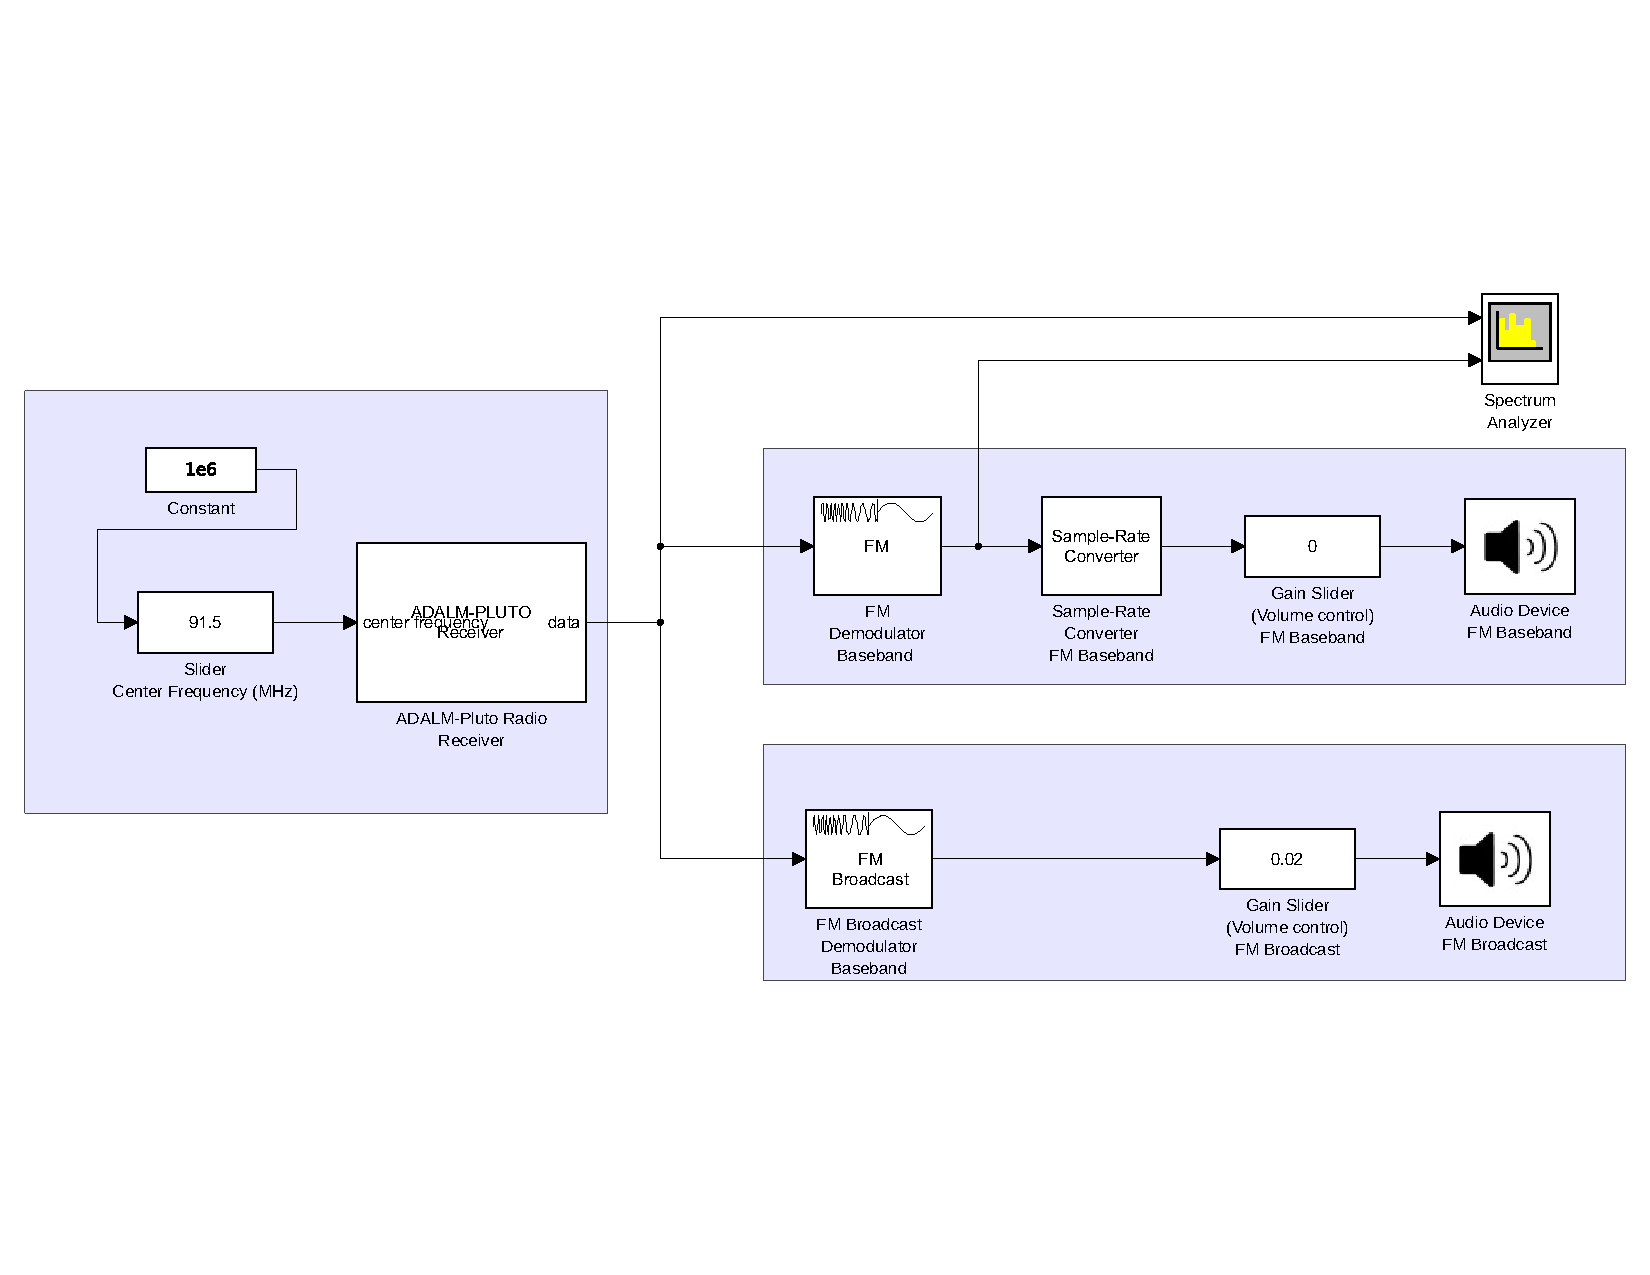
\includegraphics[trim={0cm 5cm 0cm 5cm},clip, angle=0, width=0.99\linewidth ]{pictures/lab1.pdf}
  		\caption{Izveidotā \textit{Simulink} blokshēma}\label{fig:blokshama}
\end{figure}
%
\section{Bloku parametri}
%
\begin{figure}[H]
  	 \centering
  		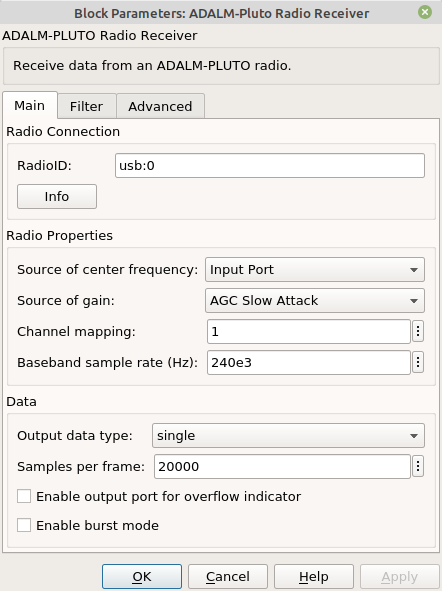
\includegraphics[trim={0cm 0cm 0cm 0cm},clip, angle=0, width=0.5\linewidth ]{pictures/adalm-pluto.png}
  		\caption{\textit{ADALM-PLUTO} bloka parametri}\label{fig:pluto}
\end{figure}
%
%
	\begin{figure}[H] % Use the t option for the alignment of the subfigures:
	\centering
		\begin{subfigure}[t]{0.45\textwidth}
		\centering
		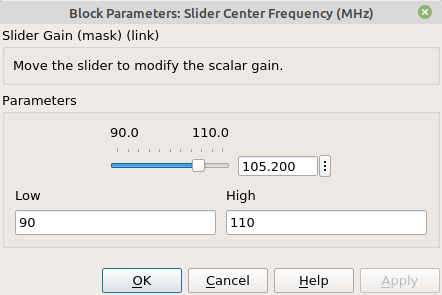
\includegraphics[trim={0cm 0cm 0cm 0cm},clip, angle=0, width=0.99\linewidth ]{pictures/fmslider.png}
		\caption{Centrālās frekvences iestatīšana}\label{fig:cf}
	\end{subfigure}
	\begin{subfigure}[t]{0.45\textwidth}
		\centering
		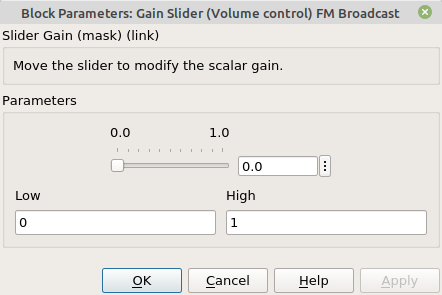
\includegraphics[trim={0cm 0cm 0cm 0cm},clip, angle=0, width=0.99\linewidth ]{pictures/gain1.png}
		\caption{Skaļuma regilēšana \textit{FM Baseband}.}\label{fig:volume1}
	\end{subfigure}
	\label{fig:pilseta_modulacija}
	\begin{subfigure}[t]{0.45\textwidth}
		\centering
		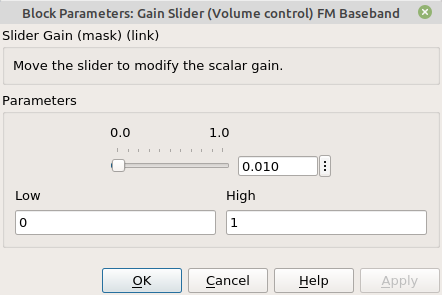
\includegraphics[trim={0cm 0cm 0cm 0cm},clip, angle=0, width=0.99\linewidth ]{pictures/gain2.png}
		\caption{Skaļuma regilēšana \textit{FM Broadcast}.}\label{fig:volume2}
	\end{subfigure}
	\caption{\textit{Slider} bloku iestatījumi}
	\label{fig:sliders}
\end{figure} 
	 % 	
\section{Novērotās oscilogrammas un spektri}
%
\begin{figure}[H]
  	 \centering
  		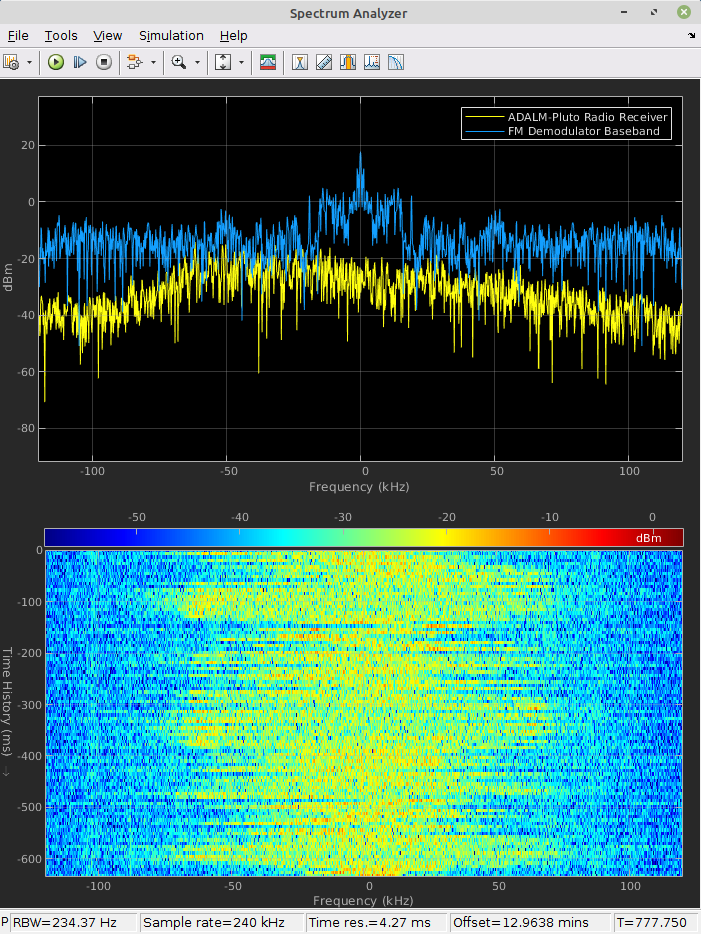
\includegraphics[trim={0cm 0cm 0cm 0cm},clip, angle=0, width=0.5\linewidth ]{pictures/spectrum_analyzer.png}
  		\caption{Spektra analizatora ekrānšāviņš}\label{fig:spectrum_analyzer}
\end{figure}
%
\section{Secinājumi}
%
Šeit ir secinājumi
%
\section{Laboratorijas darba \textit{GitHub} krātuve}
%
\begin{left}
\href{https://github.com/Clockfix/SDR\_lab1}
	{\qrcode[height=1in]{https://github.com/Clockfix/SDR\_lab1}} \ \ \ \ 
\href{https://github.com/Clockfix/SDR\_lab1}
	{https://github.com/Clockfix/SDR\_lab1}
\end{left}
%
\end{document}
